\documentclass{beamer}
\usepackage[orientation=portrait,size=a1,scale=1.4,debug]{beamerposter}
\mode<presentation>{\usetheme{ZH}}
\usepackage{chemformula}
\usepackage[utf8]{inputenc}
\usepackage[german, english]{babel} % required for rendering German special characters
\usepackage{siunitx} %pretty measurement unit rendering
\usepackage{hyperref} %enable hyperlink for urls
\usepackage{ragged2e}
\usepackage[font=scriptsize,justification=justified]{caption}
\usepackage{array,booktabs,tabularx}
\usepackage{multicol,multirow}
\usepackage{setspace}
\usepackage{graphicx,subcaption}
%%%%%%%%%%%%%%%
\newcolumntype{Z}{>{\centering\arraybackslash}X} % centered tabularx columns
\sisetup{per=frac,fraction=sfrac}
\newcommand{\specialcell}[2][c]{ \begin{tabular}[#1]{@{}c@{}}#2\end{tabular}}

\title{\huge Vehicles Chasing Each Other \\Around a Closed Path}
\author{Erdem Tuna, Halil Temurtaş, Sarper Sertel, Enes Taştan, İlker Sağlık}
\institute[ETH]{\LARGE DUAYENLER Ltd. Şti. 
}
\date{March 1, 2019}

% edit this depending on how tall your header is. We should make this scaling automatic :-/
\newlength{\columnheight}
\setlength{\columnheight}{72.5cm}

\begin{document}
\begin{frame}
\begin{columns}
	\begin{column}{.5\textwidth}
		\begin{beamercolorbox}[center]{postercolumn}
			\begin{minipage}{.98\textwidth}  % tweaks the width, makes a new \textwidth
				\parbox[t][\columnheight]{\textwidth}{ % must be some better way to set the the height, width and textwidth simultaneously
					\begin{myblock}{Company and Shareholders}
						
						Founded in September 2018 by five electrical engineering students from Middle East Technical University, DUAYENLER Ltd. Şti. is a visionary and promising new robotics start-up company. Project co-founders can be seen at \textit{Figure~\ref{fig:team}}.
												
						\subsection{Our Mission}
						Our mission is to design products for real life problems by creating innovative solutions.
						
						\subsection{Our Vision}
						Our vision is to be the frontier in robotics by intelligently automating the future world.

			\begin{figure}
				\centering
				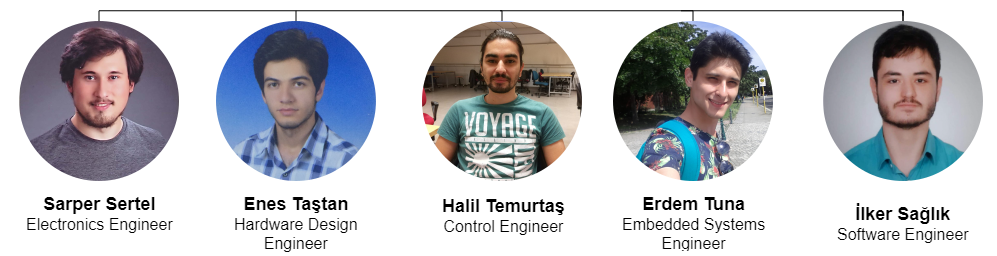
\includegraphics[width=0.8\textwidth]{img/company-tree2}
				\caption{Co-Founders of DUAYENLER Ltd. Şti.}
				\label{fig:team}
				\-\vspace{-2.0cm}
			\end{figure}
					\-\vspace{-1.5cm}
					\end{myblock} %	\vspace{.5cm}
					\vspace{-0.4em}
					\begin{myblock}{Project Description}
						The aim of the project is to design and produce a autonomous vehicle that can follow a path with varying propoerties.
						
						Throughout the project we have followed an design methodology called Agile Methodology. Agile development approach relies on rapid development and prototype production. We have also divided the project into subsections according to V-model. V chart utilized in the process can be seen at \textit{Figure~\ref{fig:vmodel}}.
						
						\begin{figure}
							\centering
							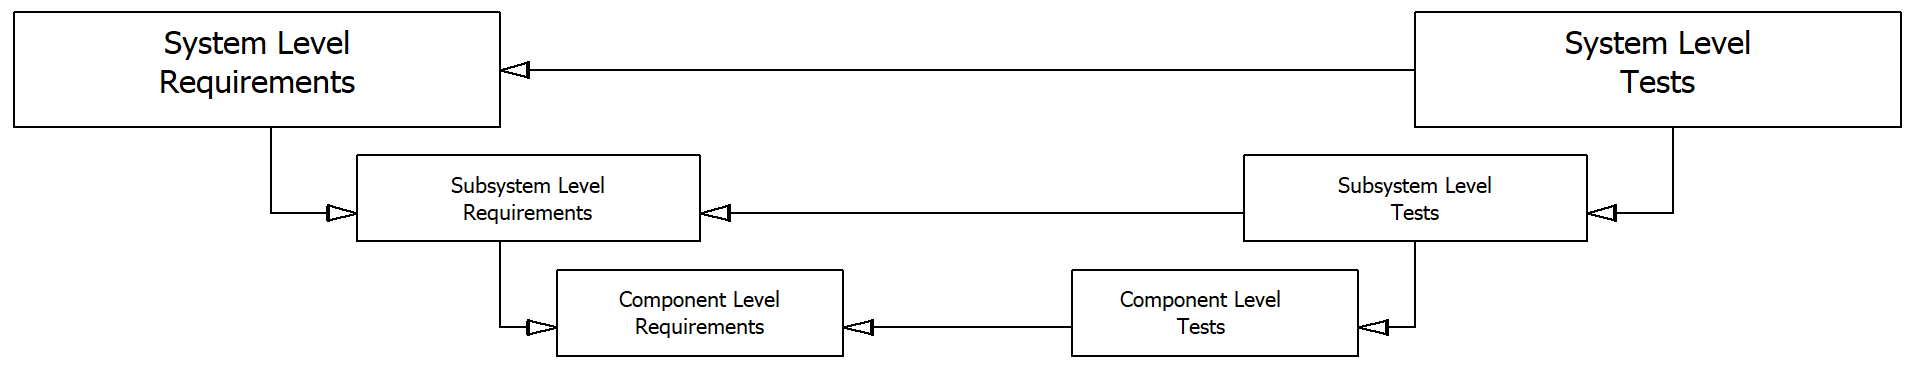
\includegraphics[width=0.9\textwidth]{img/V-model}
							\caption{V Chart for the Project Development Phase}
							\label{fig:vmodel}
						\end{figure}
						\-\vspace{-2.5cm}
					\end{myblock} 	\vspace{-0.4em}
				\begin{myblock}{Project Specifications and Requirements}
					\begin{figure}
						\centering
						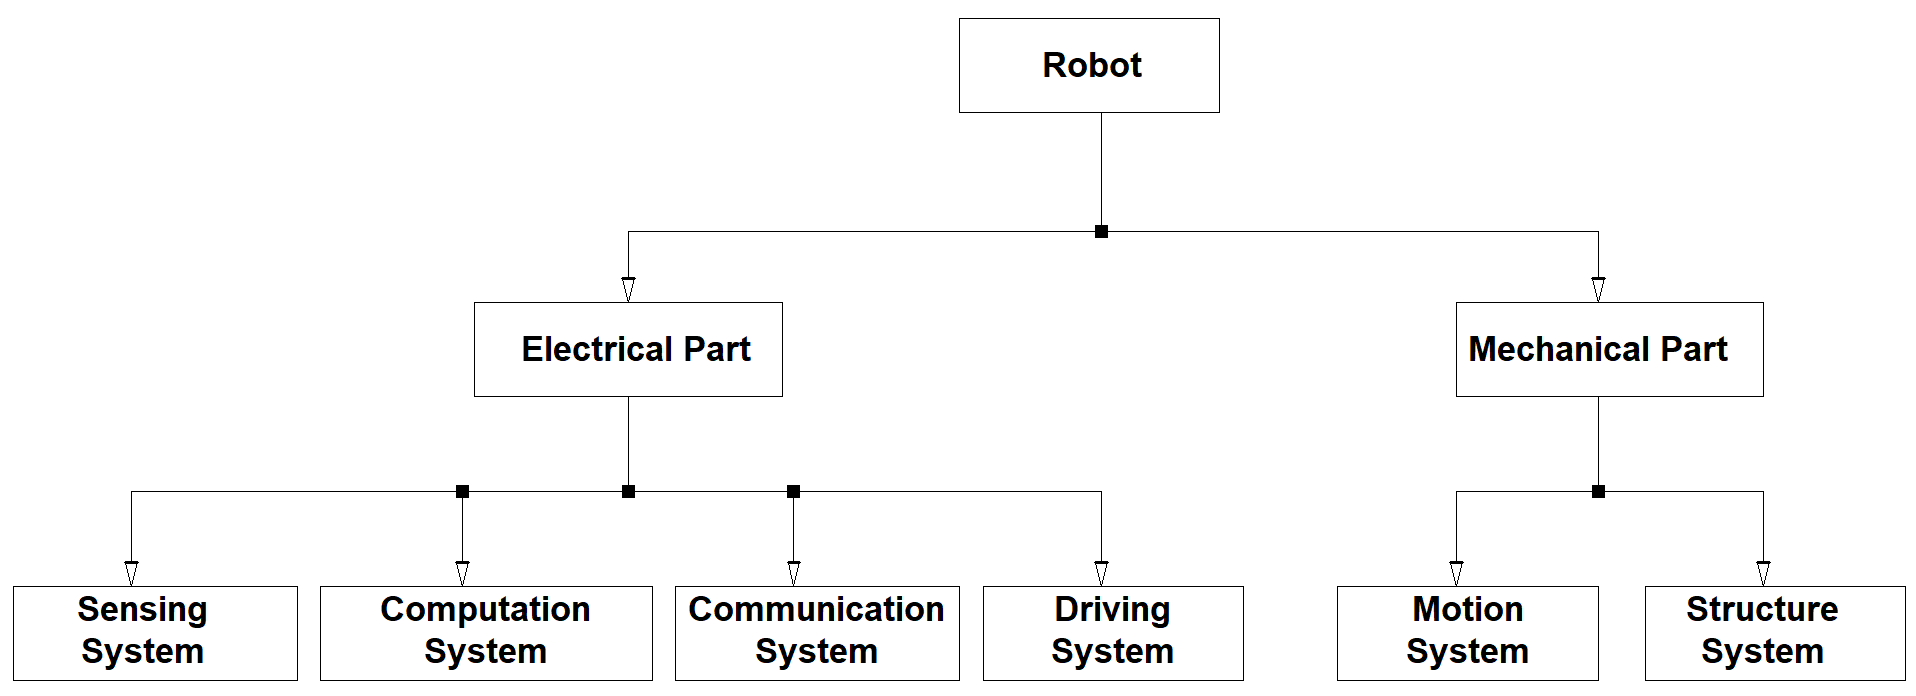
\includegraphics[width=\textwidth]{img/systems}
						\caption{System Diagram of the Project}
						\label{fig:overall-system}
					\end{figure}
				\vspace{-0.1cm}
				\begin{table}
					\caption{Requirements of the Project}
					\begin{tabular}{ll}
						%\cline{1-2}
						Project Requirements   & System Requirement \\
						\hline 
						\multirow{2}{*}{Follow path in every condition }       &  SenS: Detect lane in varying conditions       \\
						&  CmpS: Eliminate obstacles \\
						\hline
						\multirow{2}{*}{Complete path within 20 seconds}    & CmpS: Produce consistent error signal  \\
						& CmpS: Have robust controller performance  \\
						\hline
						\multirow{2}{*}{Not crash to opponent}   & SenS: Detect opponent atmost at 5 cm        \\
						& CmpS: Not be affected by the opponent \\
						\hline
						\multirow{2}{*}{Communicate with opponents}  & \multirow{2}{*}{CmnS: Follow the Handshake Protocol}      \\
						& \\
						\hline
						\multirow{2}{*}{Battery life at least 1 hour} & StrS: Supply at least 1350 mAh \\
						&  MtnS: Consume at max 15 W \\
						\hline
						\multirow{2}{*}{Production price less than  $\$200$} & StrS: Pyhsical materials cost at most  $\$200$\\
						& MtnS: Cost less than $\$35$  \\
					\end{tabular}
				\end{table} \-\vspace{-1cm}
	\end{myblock}	\vspace{-0.4em}
	\begin{myblock}{Proposed Solution}
		
		\begin{figure}
			\centering
			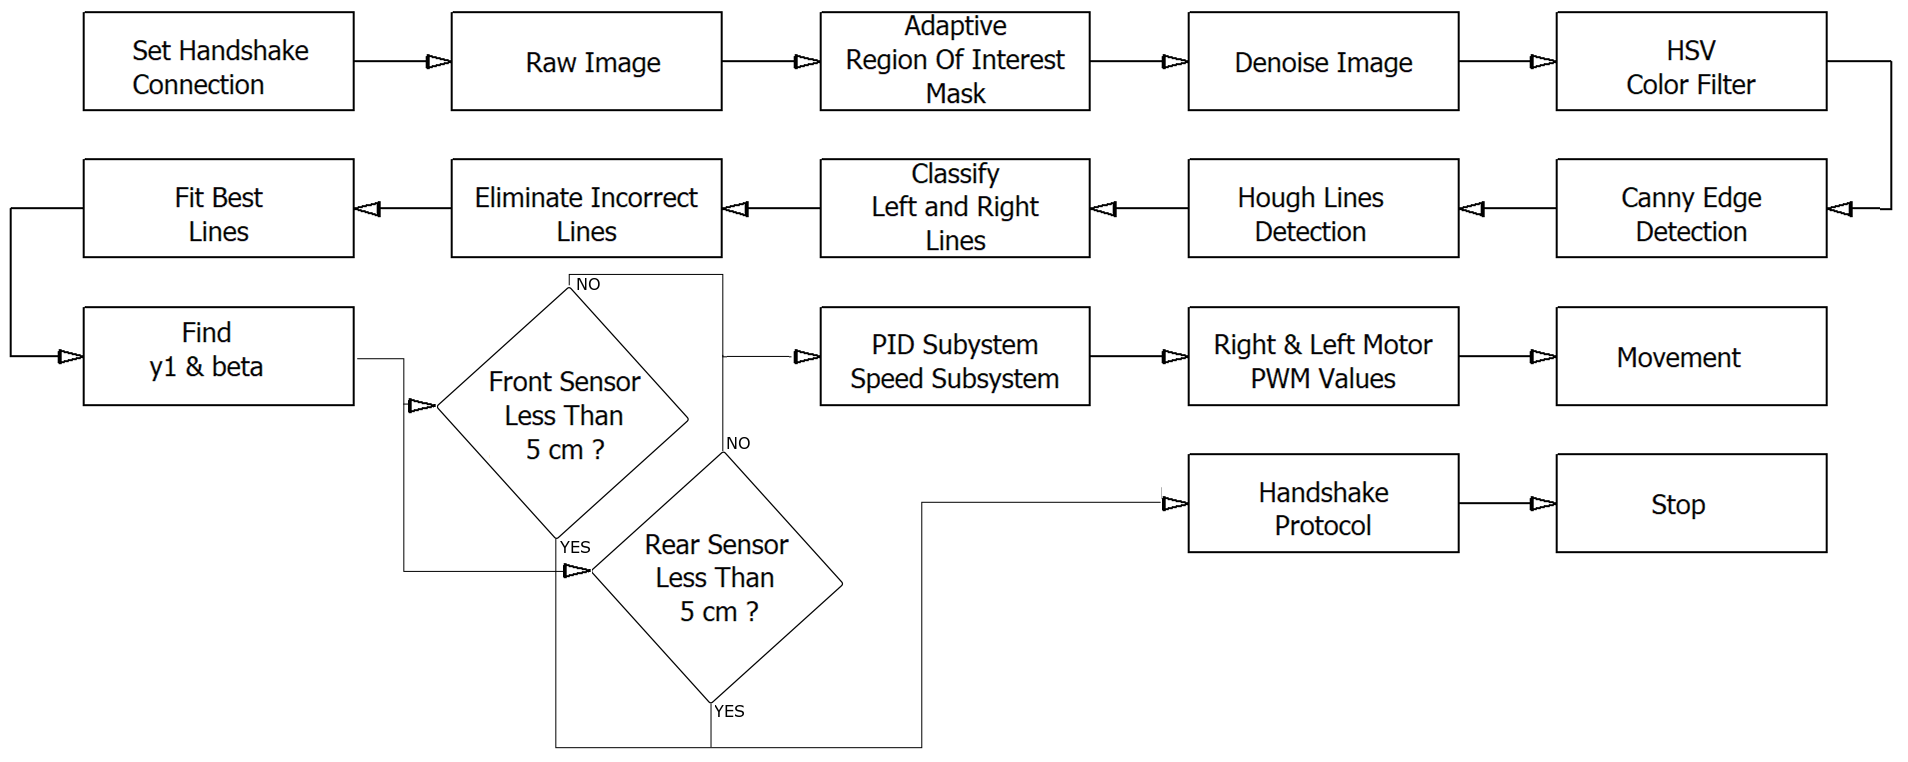
\includegraphics[width=0.85\textwidth]{img/total}
			\caption{Overall Flow Diagram of the Project}
			\label{fig:total}
		\end{figure}
	
		\begin{figure}[H]
			\centering
			\begin{subfigure}{.36\textwidth}
				\centering
				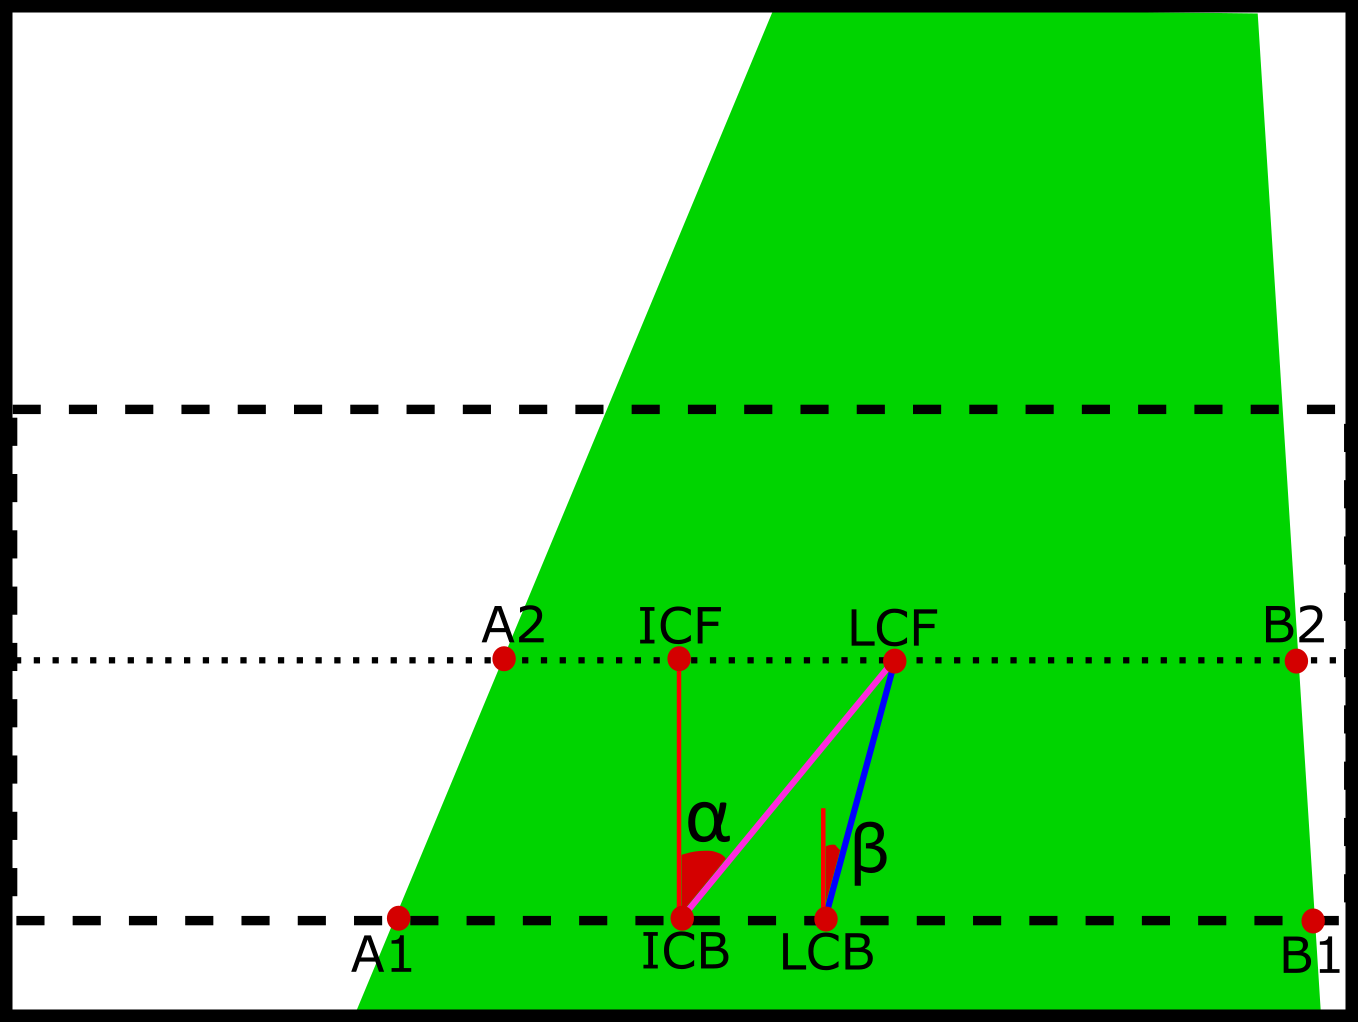
\includegraphics[width=.85\textwidth]{img/ang_cont}
				%\caption{\label{fig:ang-cont} Controllable Angle Variables }
			\end{subfigure}%
			\begin{subfigure}{.36\textwidth}
				\centering
				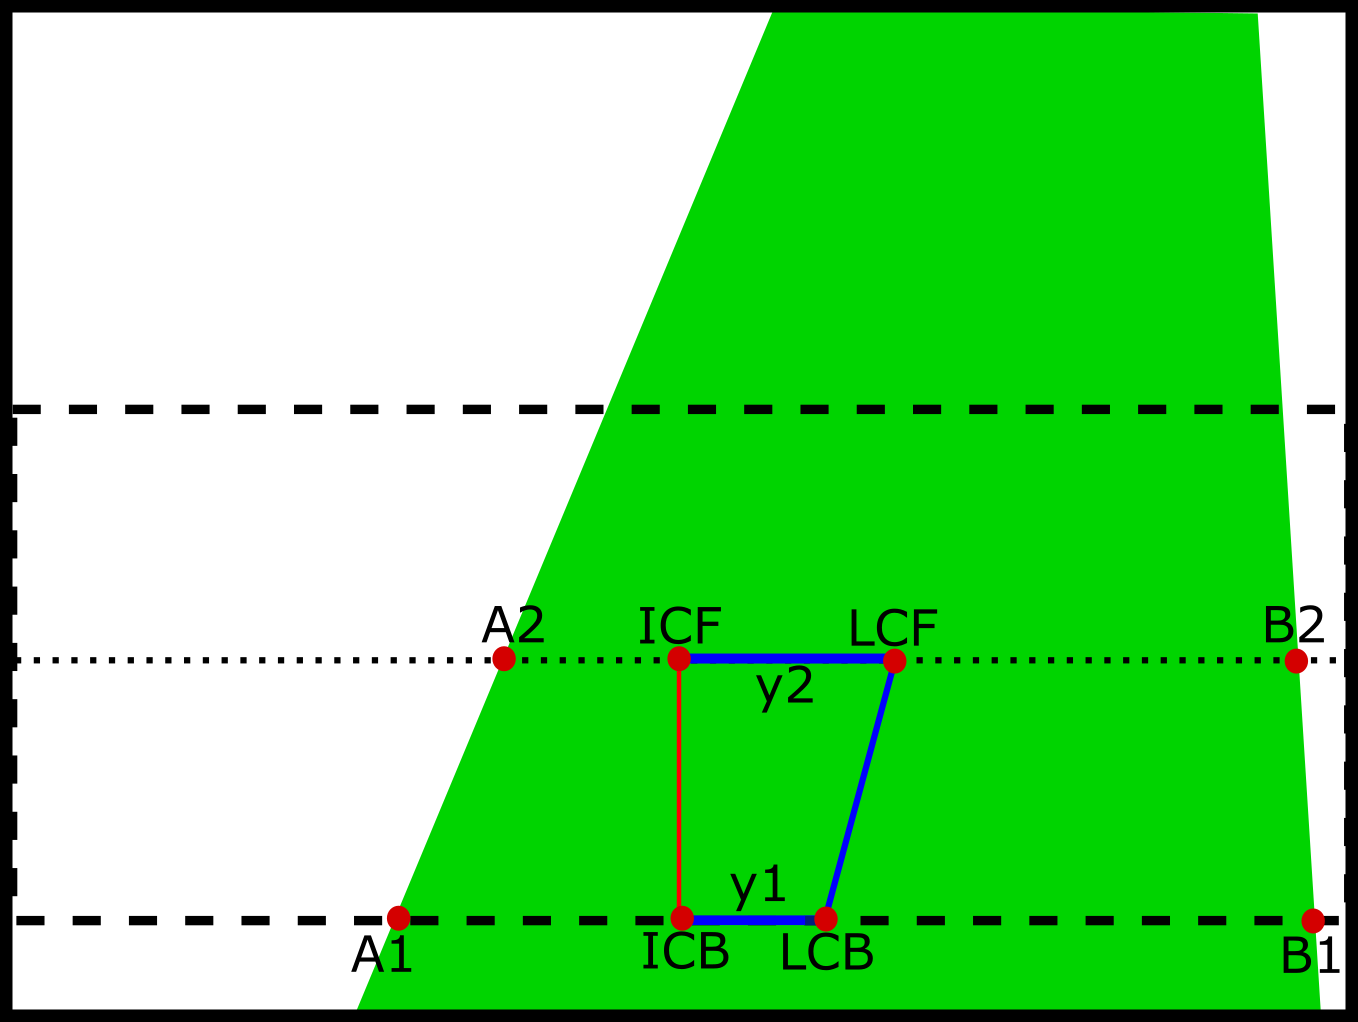
\includegraphics[width=.85\textwidth]{img/dist_cont}
				%\caption{\label{fig:dist-cont} Controllable Distance Variables}
			\end{subfigure}
			\caption{\label{fig:controlled-vars} Controlled Variables of the System }
			\-\vspace{-2.01cm}
		\end{figure}
		
	\end{myblock}	

		}\end{minipage}\end{beamercolorbox}
	\end{column}
	\begin{column}{.5\textwidth}
		\begin{beamercolorbox}[center]{postercolumn}
			\begin{minipage}{.98\textwidth} % tweaks the width, makes a new \textwidth
				\parbox[t][\columnheight]{\textwidth}{ % must be some better way to set the the height, width and textwidth simultaneously
					\begin{myblock}{Test Results}
			
				\begin{figure}
					\centering
					\includegraphics[width=0.85\textwidth]{img/pathTests}
					\caption{Test Results for the Vehicle Vision with External Disturbances}
					\label{fig:pathTests}
				\end{figure}
	
			\begin{figure}[H]
				\setlength{\unitlength}{\textwidth} 
				\centering
				\begin{subfigure}{.45\textwidth}
					\centering
					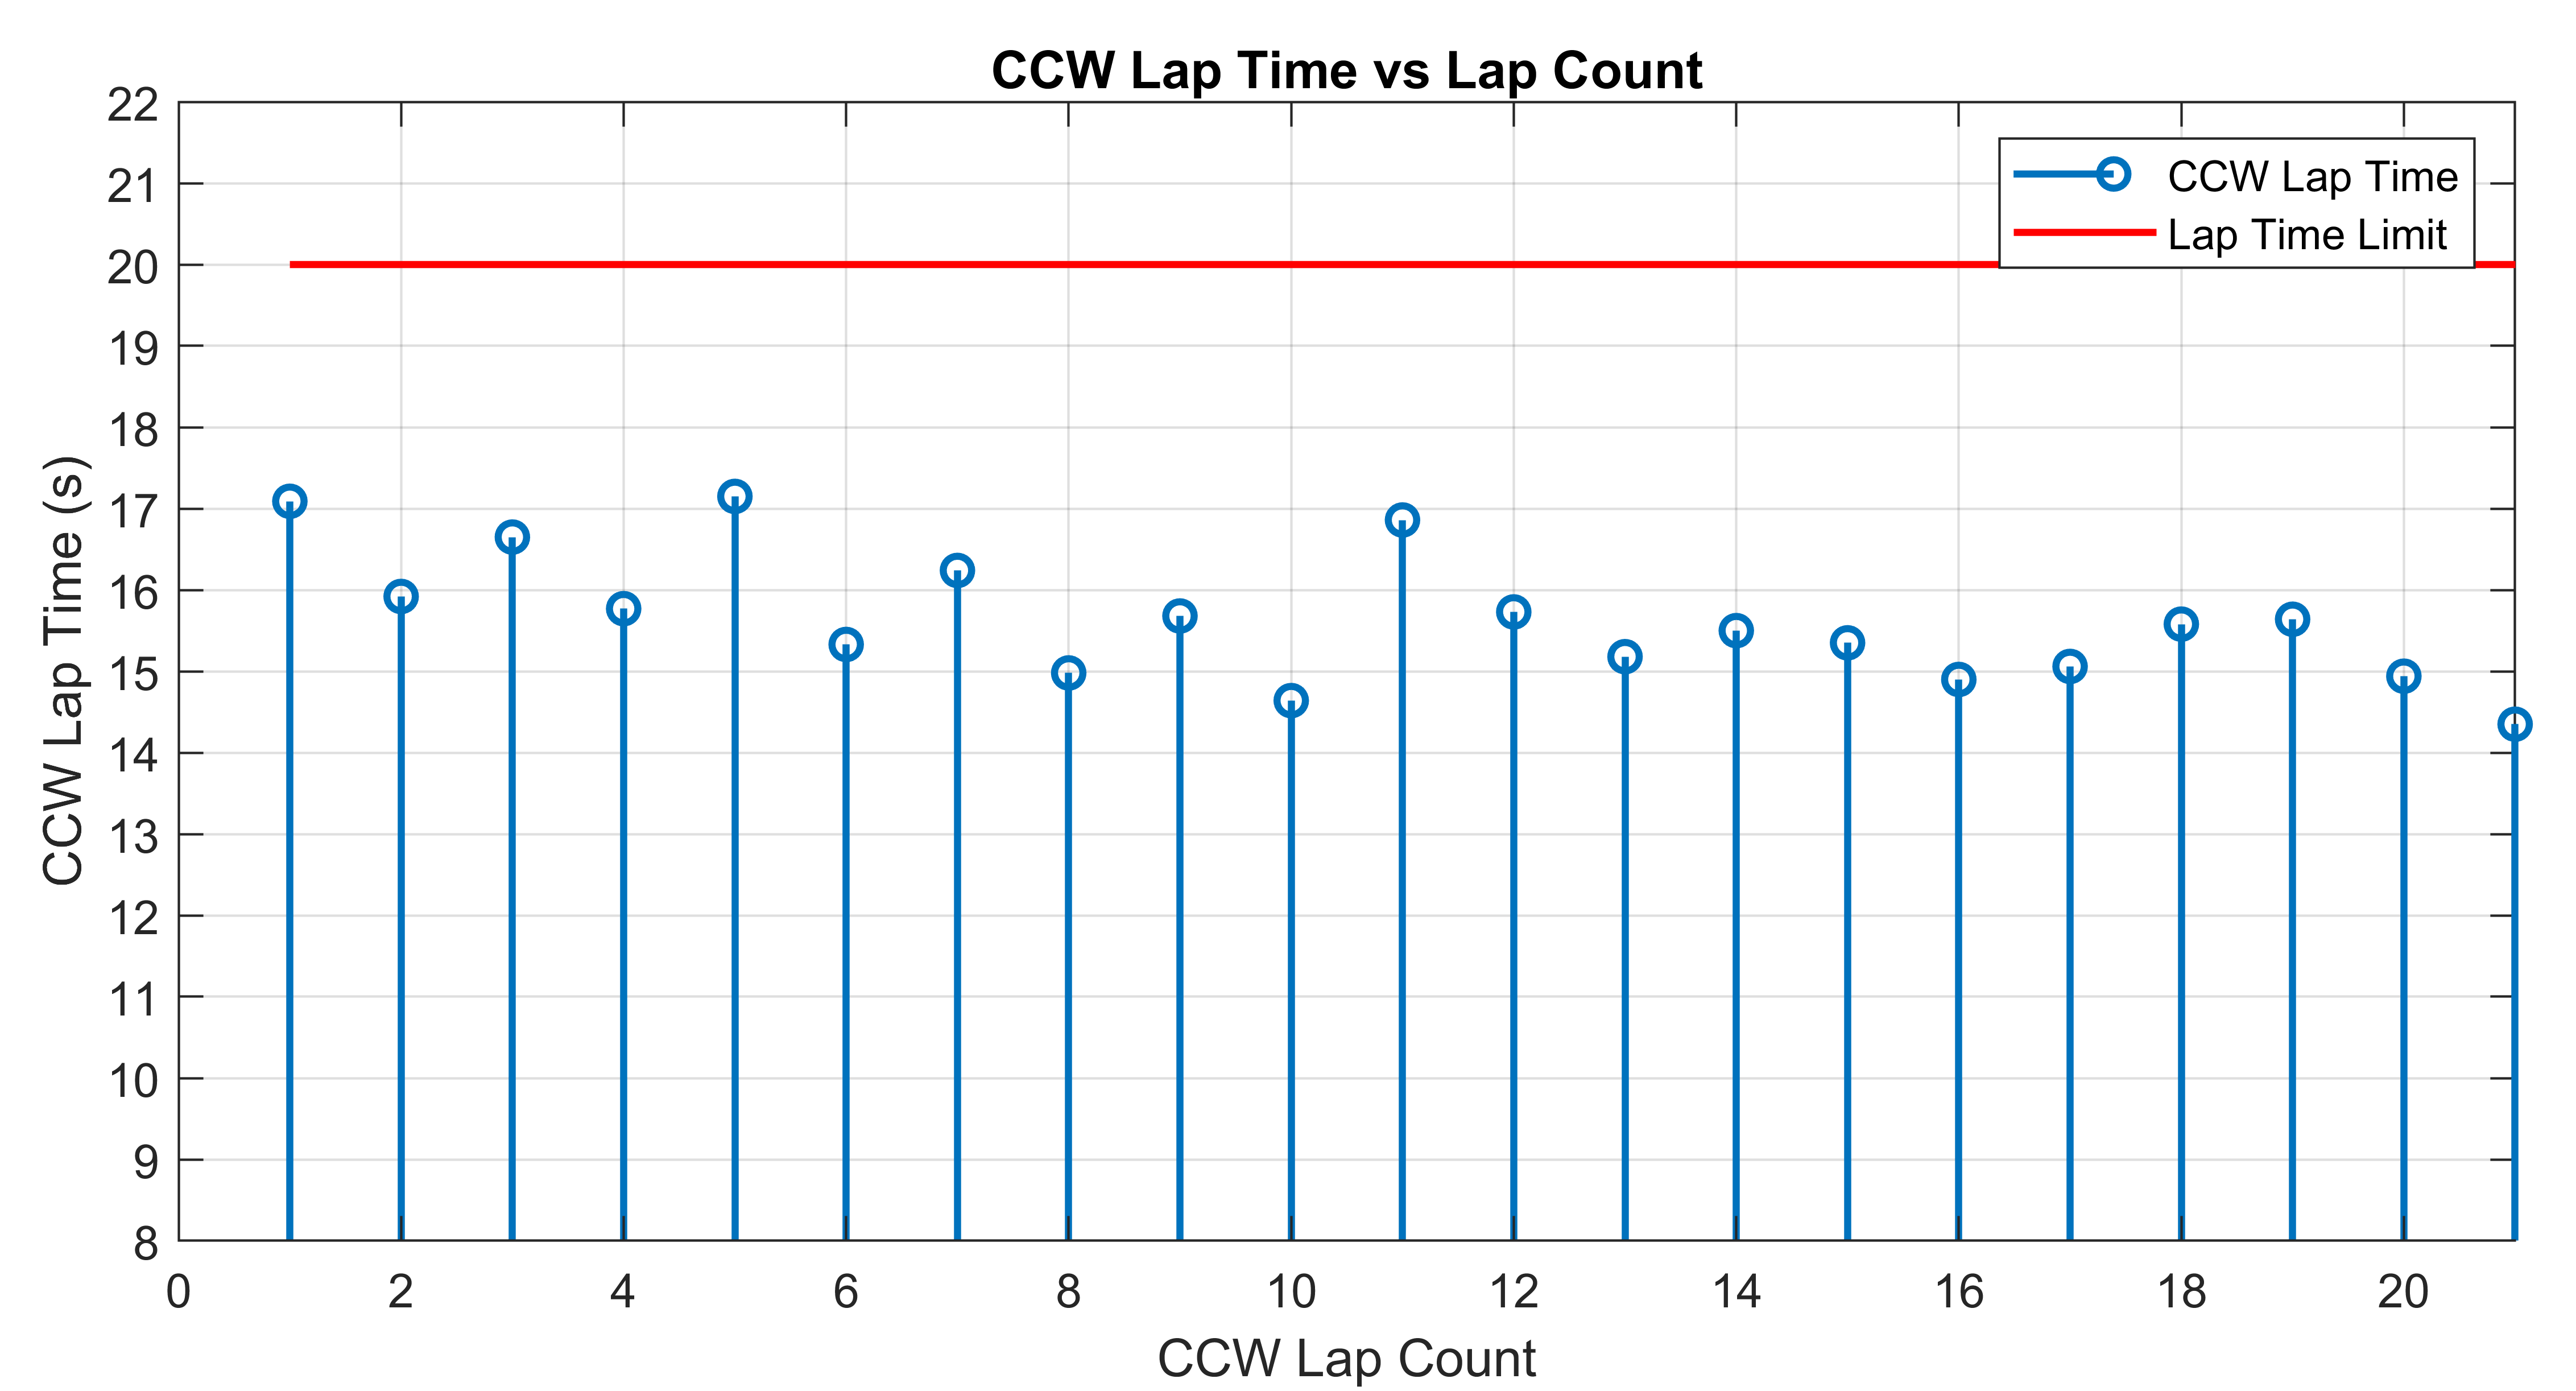
\includegraphics[width=\textwidth]{img/ccwLapTime_crop}
					%\caption{System Diagram of the Project}
				\end{subfigure}%
				\begin{subfigure}{.45\textwidth}
					\centering
				\includegraphics[width=\textwidth]{img/ProcessTime_crop}
					%\caption{System Diagram of the Project}
				\end{subfigure}
				\caption{\label{fig:test2} Left Half: CCW Lap Times for 20 Successive Laps \\ Right Half: Frame Processing Test Result }
			\end{figure}
			
			
			\begin{figure}
				\centering
				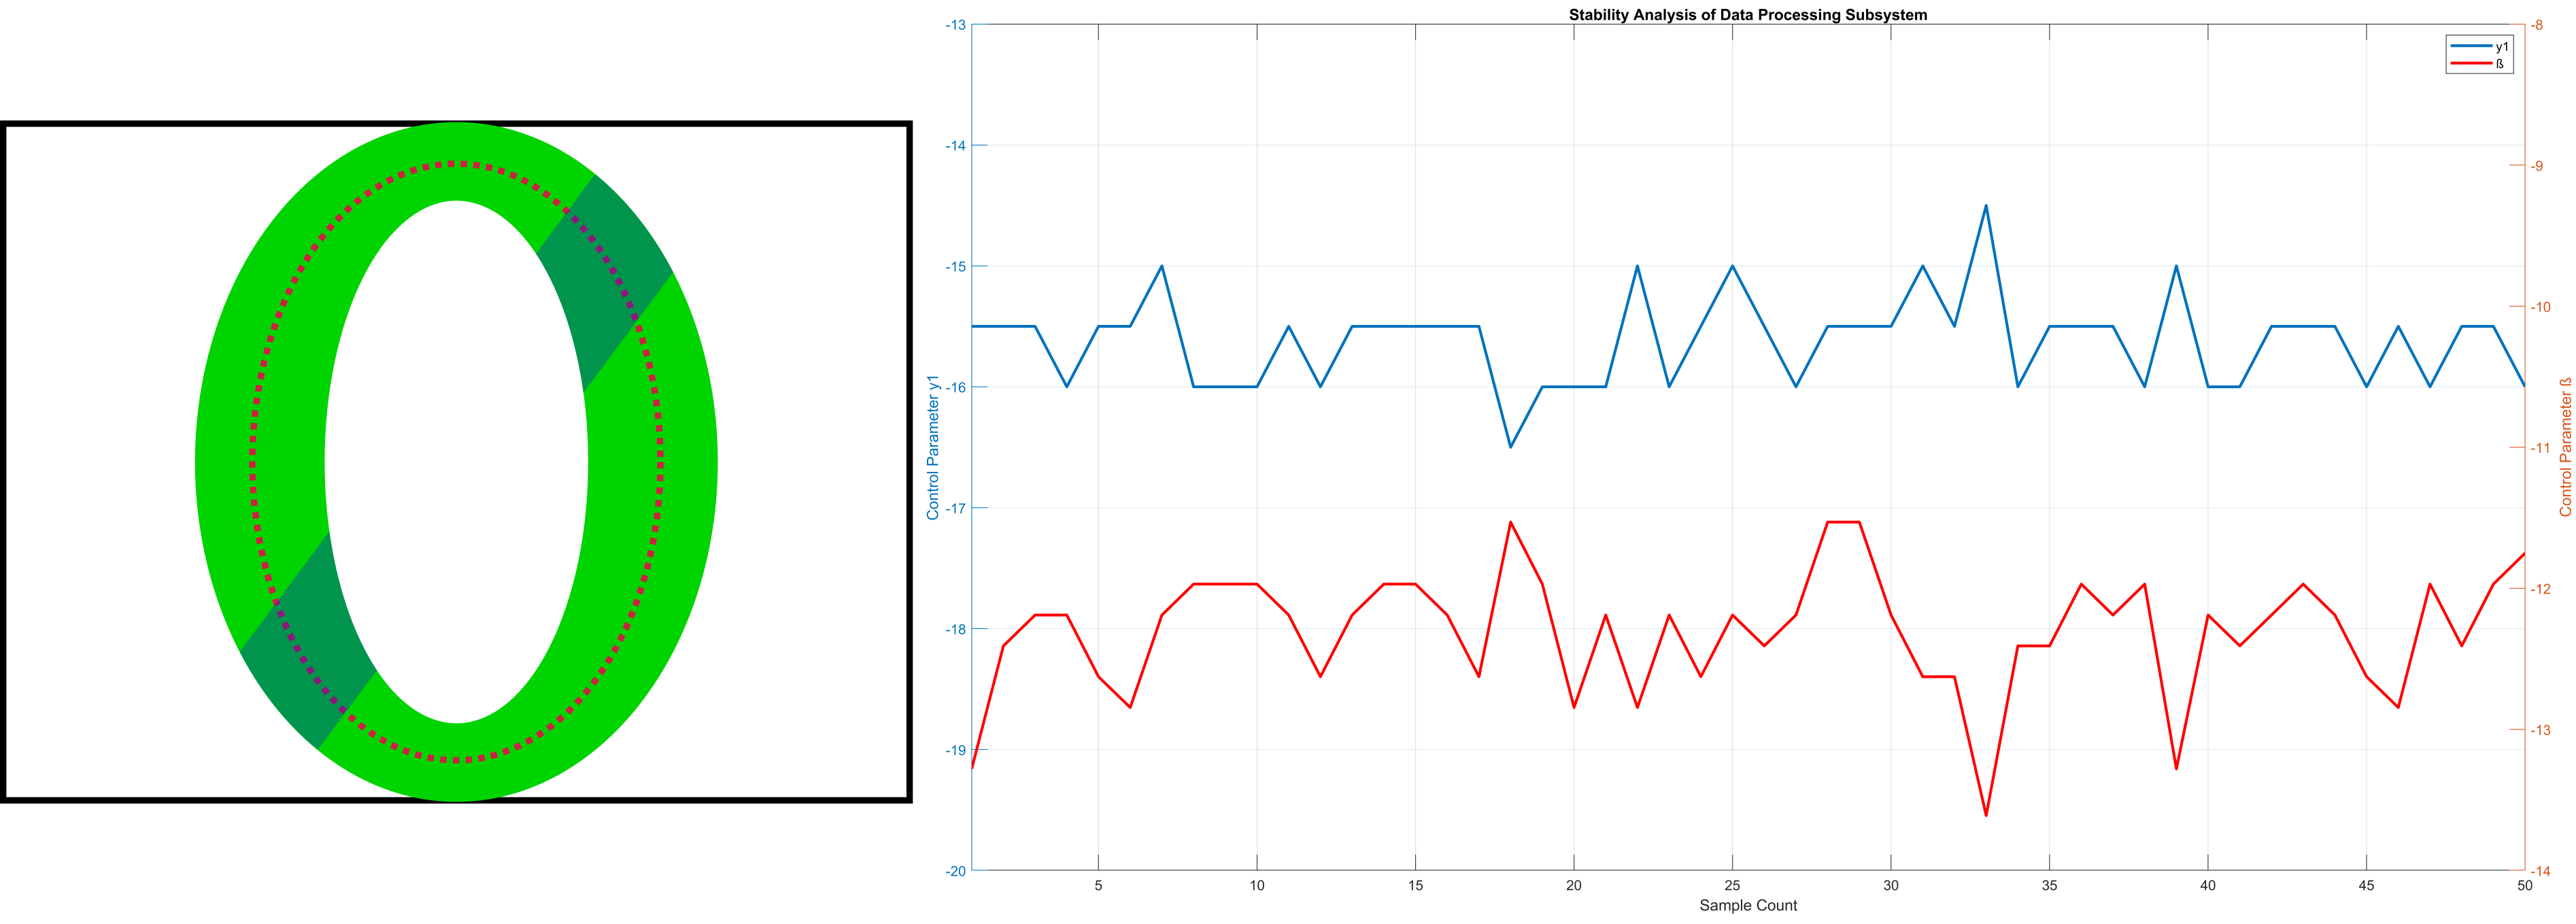
\includegraphics[width=0.8\textwidth]{img/stabilityTestS}
				\caption{Image Processing Stability Test}
				\label{fig:stabTest}
			\end{figure}
				\-\vspace{-2cm}
					\end{myblock} \vspace{-0.4em}
					\begin{myblock}{Cost Breakdown}
						\begin{table}[H]
						\centering
						\caption{Cost Analysis for the Project}
						\begin{tabular}{c c c}
							$$Component$$ & $$Number$$ & $$Total Price (in Dollar)$$  \\ \hline
							Raspberry Pi 3B & 1 & 47   \\ 
							Waveshare Raspberry Pi Camera (D) & 1 & 22   \\ 
							Chassis Components & 1 & 13   \\ 
							Arduino Nano & 1 &  4.8 \\ 
							Polulu 150:1 6 V 200 RPM DC Motor & 2 & 42 \\ 
							Bond Silicon Wheel & 2 & 8 \\ 
							Motor Driver and Voltage Regulator & 1 &  4 \\ 
							Xiaomi 10000 mAh Mi Powerbank (Ver 3) & 1 & 12 \\ 
							ProFuse 11.1 V 1750 mAh Li-po Battery  & 1 & 23 \\ 
							Polulu VL6180X ToF Distance Sensor & 2 & 17 \\
							LED headlight/LED & - & 0.2 \\ 
							Styrofoam, Glue $\&$ Cardboard & - & 6.5 \\ \hline
							Total Project & - & 199.5 
						\end{tabular} 
						\label{tab:cost}
					\end{table}
				\-\vspace{-1cm}
					\end{myblock} \vspace{-0.4em}
				\begin{myblock}{Power Analysis}
					\begin{table}[H]
						\centering
						\caption{Estimated Cost Analysis for the Project}
						\begin{tabular}{c c c c c}
							$$Component$$ & $$\specialcell{Current\\ (Avg),A}$$ & $$\specialcell{Power\\(Avg),W}$$ & $$\specialcell{Current\\(Max),A}$$ & $$\specialcell{Power\\(Max),W}$$ \\ \hline
							Raspberry Pi 3B & 0.85 & 4.25 & 2.5 & 12.5  \\
							Arduino Nano & 80m &  0.4 & 0.2 & 1 \\ 
							DC Motors \& Motor Driver & 0.35 & 4.2 & 0.95 & 11.4 \\ 
							Distance Sensor & 19m & 62.7m & 40m & 132m \\ \hline
							Total  &  1.349 & 8.9127 & 3.69 & 25.032         
						\end{tabular} 
						\label{tab:power}
					\end{table}
					\-\vspace{-1cm}
				\end{myblock} \vspace{-0.4em}
					\begin{myblock}{Deliverables}
						Deliverables of the product are listed as follows;
						\begin{multicols}{2}
							\begin{itemize}
								\item KOBRA 6.5  
								\item Race Track 
								\item Flash stick with sofware 
								\item User Manual 
								\item Micro USB Cable
							\end{itemize} 
						\end{multicols}
					\-\vspace{-1.5cm}
					\end{myblock} \vspace{-0.4em}
				\begin{myblock}{Acknowledge}
					DUAYENLER would like to thank METU Physics Society and Ali Aslantürk for their valuable contributions.
				\end{myblock} 
					%\begin{myblock}{References}
					%	\footnotesize
					%	\bibliographystyle{ieeetr}
					%	\bibliography{./bib}
					%\end{myblock}
		}\end{minipage}\end{beamercolorbox}
	\end{column}
\end{columns}
\end{frame}
\end{document}
